\part{Scheduling}
Concurrent programs exhibit non-determinism, and a real-time system needs to restrict this non-determinism through scheduling. A scheduling scheme provides two key features:
\begin{enumerate}
\item An algorithm for ordering the use of system resources
\item A way to predict the worst-case behavior of the system when the scheduling algorithm is applied.
\end{enumerate}

There are \textbf{static} (prediction only before execution) and \textbf{dynamic} (run-time decisions are used) schemes for scheduling. The focus in this course is on static schemes, specifically \textit{preemptive priority-based schemes on a single-processor system}. The task with the highest priority will always run, unless it is suspended or delayed for some reason. The two features above can be re-stated as:
\begin{enumerate}
\item Priority assignment algorithm
\item Schedulability test
\end{enumerate}

\subsection{What is non-preemptive scheduling (cyclic executive)}
What is non-preemptive scheduling:
\begin{itemize}
\item Fixed set of tasks with fixed periods. 
\item Consists of a table of procedure calls, the majority cycle, compromised of smaller minor cycles with fixed duration.
\item At run-time, no task can run concurrently, therefore mutual exclusion is guaranteed and we do not need synchronization primitives such as semaphores.
\item All task periods must be a multiple of the minor cycle period.
\end{itemize}
 
 What are some of its drawbacks?
 \begin{itemize}
 \item  Difficult to incorporate sporadic tasks.
\item Difficult to construct
\item Difficult to incorporate tasks with long periods
\item "Large" tasks will need to be split up into several procedures, which may hurt the code quality and make it more error-prone.
 \end{itemize}
 
\section{Task-based scheduling}
Tasks exist at run-time, supported by real-time OS or run-time kernel. Each task is either \textit{runnable/running}, \textit{suspended waiting for timing event} or \textit{suspended waiting for non-timing event}. There are different approaches to Task-based scheduling
\begin{itemize}
\item Fixed-Priority Scheduling (FPS)
\item Earliest Deadline First (EDF)
\item Value-Based Scheduling (VBS)
\end{itemize}

\subsubsection{Fixed-Priority Scheduling}
Most widely used and main focus in this course. Each task has a static priority computed pre-run-time and the runnable tasks are executed in the order determined by their priority.

With priority-based scheduling, a high-priority task may be released during the executing of a lower priority one. In a \textbf{preemptive} scheme, there will be an immediate switch to the higher-priority task. With \textbf{non-preemption}, the lower priority task will be allowed to complete before the other executes.Preemptive allows for more reactive high-priority tasks. \textbf{Cooperative dispatching (deferred preemption)} is a hybrid of the two. EDF and VBS can also either take a preemptive or non-preemptive approach.

\subsection{Scheduling characteristics}
\begin{itemize}
\item \textbf{Sufficient scheduling} - passing the test results in a program that meet deadlines.
\item \textbf{Necessary scheduling} - failing the scheduling test guarantees that deadlines will be missed.
\item \textbf{Exact scheduling} - Necessary and sufficient
\item \textbf{Sustainable scheduling} - system stays schedulable if conditions improve.
\end{itemize}

\subsection{Simple task model}
Simple Task Model makes the following assumptions:
\begin{itemize}
\item The application is assumed to consist of a fixed set of tasks
\item All tasks are periodic, with known periods.
\item The tasks are completely independent
\item All system's overheads, context-switching times and so on are ignored (i.e. assumed to have zero cost)
\item All tasks have a deadline equal to their period, that is each task must complete before it is next released
\item All tasks have a fixed worst-case execution time.
\end{itemize}

\subsection{Standard Notation}
\begin{itemize}
\item \textbf{C} - Worst-case computation time of task
\item \textbf{D} - Deadline of the task
\item \textbf{I} - The interference time of the task
\item \textbf{N} - Number of tasks in the system
\item \textbf{P} - Priority assigned to the task (if applicable)
\item \textbf{R} - Worst-case response time of the task
\item \textbf{T} - Minimum time between task releases, jobs (task period). In simple task model \texttt{T=D}
\item \textbf{U} utilization of each task, equal to \texttt{C/T}
\item \textbf{a-z} The name of the task.
\end{itemize}

\subsection{Rate Monotonic Priority Assignment}
Each task is assigned a unique priority based on its period; the shorter the period the higher the priority. I.e. for two tasks i and j
\begin{equation}
T_i<T_j \implies P_i > P_j
\end{equation}
This assignment is optimal in the sense that if any task can be scheduled, using preemptive scheduling, with a fixed-priority assignment scheme, then the given task set can also be scheduled with a rate monotonic assignment scheme. Note that priority 1 is lowest (least) priority.

\subsection{Utilization-Based Analysis}
This method only works for tasks following the simple task model as \texttt{D=T} must be affirmed. It is a simple \textit{sufficient} but \textbf{not} \textit{necessary} schedulability test
\begin{align}
U = \sum_{i=1}^N\frac{C_i}{T_i}\leq N(2^\frac{1}{N}-1) \\
U\leq 0.69 \text{ as } N\to\infty
\end{align}

\subsection{Response-Time Analysis}
Here task \texttt{i}'s worst-case response time \textbf{R} is calculated first and then checked trivially with it's deadline 
\begin{align}
R_i\leq D_i \\
R_i = C_i + I_i
\end{align}
where $I_i$ is the interference on task i from higher priority tasks.

\subsubsection{Calculating R}
During R, each higher priority task j will execute a number of times:
\begin{align}
\text{Number of Releases}=\ceil*{\frac{R_i}{T_j}}
\end{align}
Total interference from task j is then given by:
\begin{align}
    \ceil*{\frac{R_i}{T_j}}C_j
\end{align}
From this we get the \textbf{Response Time Equation}
\begin{align}
R_i = C_i +\sum_{j\in hp(i)}\ceil*{\frac{R_i}{T_j}}C_j
\end{align}
where $hp(i)$  is the set of tasks with higher priority than task i. Solve the Response Time Equation with the recurrence relationship:
\begin{align}
w_i^{n+1} = C_i + \sum_{j\in hp(i)}\ceil*{\frac{w_i^n}{T_j}}C_j
\end{align}
The set of values $w_i^0$ , ---,$w_i^n$, ... is monotonically non-decreasing. When 
\begin{align}
w_i^n=w_i^{n+1}
\end{align}
the solution to the equation has been found. $w_i^0$ must not be greater than $R_i$ , it can e.g. be 0 or $C_i$ . 

\subsection{Example}
\begin{figure}[H]
\centering
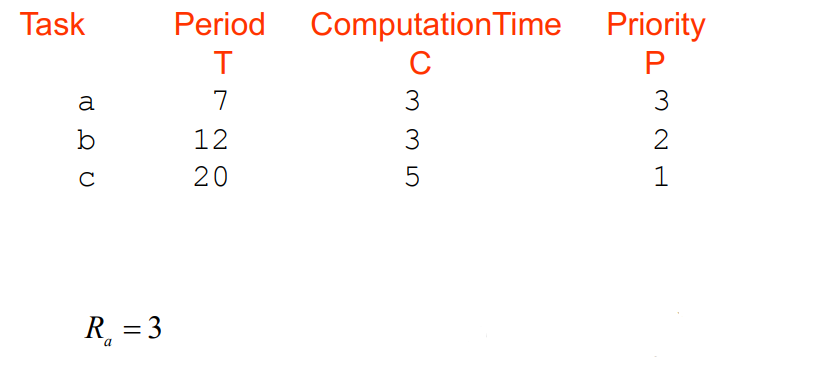
\includegraphics[width=0.9\linewidth]{figures/Scheduling/Response Time Analysis/example.PNG}
\end{figure}
\begin{align}
    w_b^0 = 3 \\
    w_b^1 = 3 + \ceil*{\frac{3}{7}}3 = 6 \\
    w_b^2 = 3 + \ceil*{\frac{6}{7}}3 = 6\\
    R_b = 6
\end{align}
\begin{align}
w_c^0 = 5
w_c^1 = 5 + \ceil*{\frac{5}{12}}3 + \ceil*{\frac{5}{7}}3 = 11 \\
w_c^2 = 5 + \ceil*{\frac{11}{12}}3 + \ceil*{\frac{11}{7}}3 = 14 \\
w_c^3 = 5 + \ceil*{\frac{14}{12}}3 + \ceil*{\frac{14}{7}}3 = 17 \\
w_c^4 = 5 + \ceil*{\frac{17}{12}}3 + \ceil*{\frac{17}{7}}3 = 20 \\
w_c^5 = 5 + \ceil*{\frac{20}{12}}3 + \ceil*{\frac{20}{7}}3 = 20 \\
R_c = 20
\end{align}
We have that for both task a, taks b and task c, $R_i\leq D_i=T_i$ 

\subsubsection{Summary}
Response time analysis is \textbf{sufficient and necessary (exact)}. If the task set passes the test they will meet all their deadlines and if they fail the test then at run-time a task will miss its deadline under the assumption that computation time estimations themselves are not pessimistic)

\subsection{Task Interactions and Blocking}
If a task is suspended waiting for a lower-priority task to complete some required computation then the priority model is in some sense being \textit{undermined}. It is said to suffer \textbf{priority inversion} and the high-priority task waiting for low-priority is said to be \textbf{blocked}. To show this, consider an example where four periodic tasks a,b,c and d and two resources Q and V are at play:
\begin{figure}[H]
    \centering
    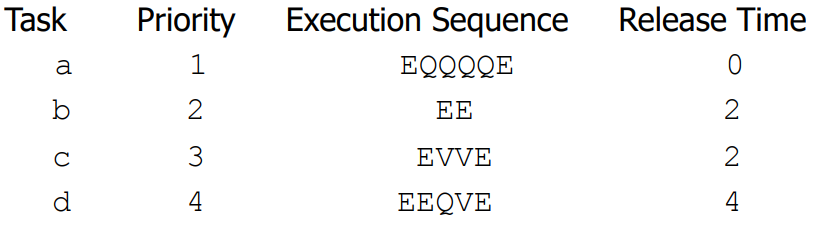
\includegraphics[width=0.9\linewidth]{figures/Scheduling/Priority Inversion/Overview.PNG}
\end{figure}
\begin{figure}[H]
    \centering
    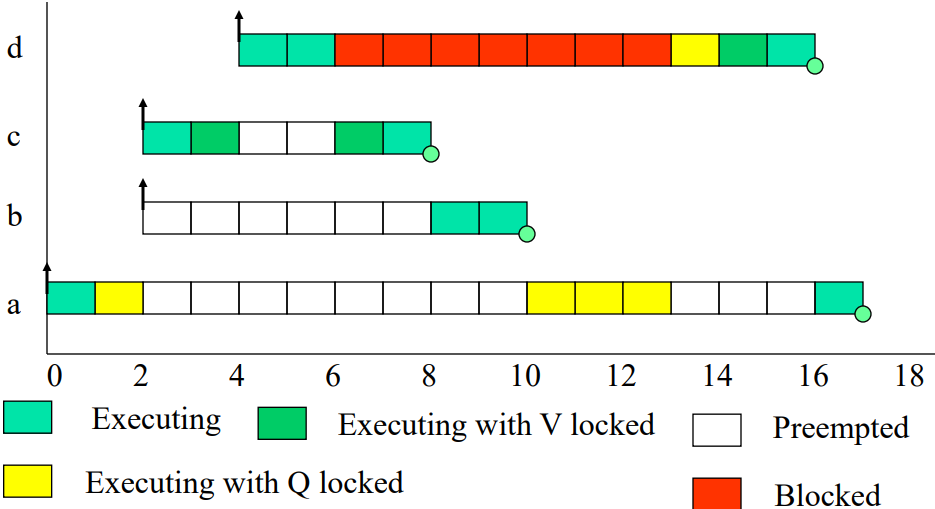
\includegraphics[width=0.9\linewidth]{figures/Scheduling/Priority Inversion/Sequence.PNG}
\end{figure}
What we see here is that if task $p$ is blocking task $q$, then $p$ runs with $q$ 's priority. Above d runs with a's priority.

\subsection{Priority Ceiling Protocols}
A priority ceiling protocol avoids \textbf{unbounded priority inversion} and deadlock. Each shared resource is assigned a ceiling priority equal to the highest priority of any task that can lock it. There are two forms
\begin{itemize}
\item Original Ceiling Priority Protocol (OCPP)
\item Immediate ceiling priority protocol (ICPP)
\end{itemize}
If we are on a single processor, the protocol ensures the following
\begin{itemize}
\item High-priority task can be blocked at most once during its execution by lower-priority tasks.
\item Deadlocks are prevented
\item Transitive blocking is prevented
\item Mutual exclusive access to resources is ensured by the protocol itself.
\end{itemize}

\subsubsection{OCPP}
\begin{itemize}
\item Each task has a static default priority assigned.
\item  Each resource has a static ceiling value defined, this is the maximum priority of the tasks that use it.
\item A task has a dynamic priority that is the maximum of its own static priority and any it inherits due to it blocking higher-priority tasks,
\item A task can only lock a resource if its dynamic priority is higher than the ceiling of any currently locked resource excluding any that it has already locked itself.
\end{itemize}
\begin{figure}[H]
\centering
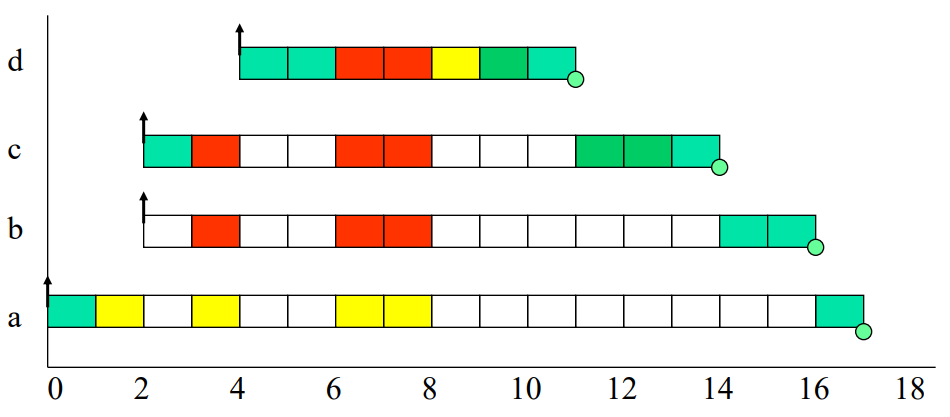
\includegraphics[width=0.9\linewidth]{figures/Scheduling/Priority Inversion/OCPP.PNG}
\end{figure}

\subsubsection{ICPP}
\begin{itemize}
\item Each task static default priority
\item Resource has static ceiling value defined, this is maximum priority of the tasks that use it.
\item A task has a dynamic priority that is the maximum of static and ceiling value of any resource it has locked.
\item Consequence of ICPP; task will only suffer block at the very beginning of its execution.
\item Consequence of ICPP; once task starts executing, all resources it needs must be free; if they were not, then some task would have an equal or higher priority and the task's execution would be postponed.
\end{itemize}
\begin{figure}[H]
\centering
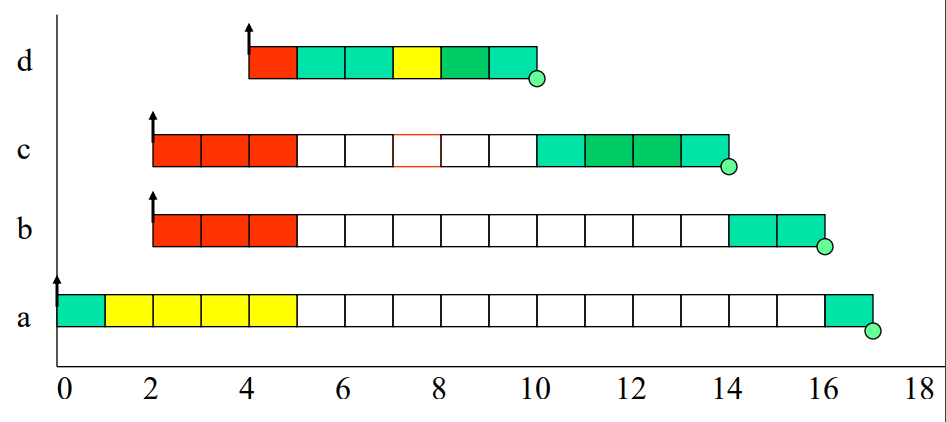
\includegraphics[width=0.9\linewidth]{figures/Scheduling/Priority Inversion/ICPP.PNG}
\end{figure}

\subsubsection{OCPP versus ICPP}
Worst-case behavior is identical but are some differences:
\begin{itemize}
\item ICPP easier to implement as blocking relationships need not be monitored.
\item ICPP leads to less context switching
\item ICPP requires more priority movements as this happens with all resource useage.
\item OCPP changes priority only if an actual block has occurred.
\end{itemize}

